\documentclass[journal,12pt,twocolumn]{IEEEtran}

\usepackage{setspace}
\usepackage{gensymb}
\singlespacing
\usepackage[cmex10]{amsmath}
\usepackage{multirow}
\usepackage{amsthm}
\usepackage{mathrsfs}
\usepackage{txfonts}
\usepackage{stfloats}
\usepackage{bm}
\usepackage{cite}
\usepackage{cases}
\usepackage{subfig}

\usepackage{longtable}

\usepackage{enumitem}
\usepackage{mathtools}
\usepackage{steinmetz}
\usepackage{tikz}
\usepackage{circuitikz}
\usepackage{verbatim}
\usepackage{tfrupee}
\usepackage[breaklinks=true]{hyperref}
\usepackage{graphicx}
\usepackage{tkz-euclide}

\usetikzlibrary{calc,math}
\usepackage{listings}
    \usepackage{color}                                            %%
    \usepackage{array}                                            %%
    \usepackage{longtable}                                        %%
    \usepackage{calc}                                             %%
    \usepackage{multirow}                                         %%
    \usepackage{hhline}                                           %%
    \usepackage{ifthen}                                           %%
    \usepackage{lscape}     
\usepackage{multicol}
\usepackage{chngcntr}

\DeclareMathOperator*{\Res}{Res}

\renewcommand\thesection{\arabic{section}}
\renewcommand\thesubsection{\thesection.\arabic{subsection}}
\renewcommand\thesubsubsection{\thesubsection.\arabic{subsubsection}}

\renewcommand\thesectiondis{\arabic{section}}
\renewcommand\thesubsectiondis{\thesectiondis.\arabic{subsection}}
\renewcommand\thesubsubsectiondis{\thesubsectiondis.\arabic{subsubsection}}


\hyphenation{op-tical net-works semi-conduc-tor}
\def\inputGnumericTable{}                                 %%

\lstset{
%language=C,
frame=single, 
breaklines=true,
columns=fullflexible
}
\graphicspath{{./Figures/}}
\begin{document}


\newtheorem{theorem}{Theorem}[section]
\newtheorem{problem}{Problem}
\newtheorem{proposition}{Proposition}[section]
\newtheorem{lemma}{Lemma}[section]
\newtheorem{corollary}[theorem]{Corollary}
\newtheorem{example}{Example}[section]
\newtheorem{definition}[problem]{Definition}

\newcommand{\BEQA}{\begin{eqnarray}}
\newcommand{\EEQA}{\end{eqnarray}}
\newcommand{\define}{\stackrel{\triangle}{=}}
\bibliographystyle{IEEEtran}
\raggedbottom
\setlength{\parindent}{0pt}
\providecommand{\mbf}{\mathbf}
\providecommand{\pr}[1]{\ensuremath{\Pr\left(#1\right)}}
\providecommand{\qfunc}[1]{\ensuremath{Q\left(#1\right)}}
\providecommand{\sbrak}[1]{\ensuremath{{}\left[#1\right]}}
\providecommand{\lsbrak}[1]{\ensuremath{{}\left[#1\right.}}
\providecommand{\rsbrak}[1]{\ensuremath{{}\left.#1\right]}}
\providecommand{\brak}[1]{\ensuremath{\left(#1\right)}}
\providecommand{\lbrak}[1]{\ensuremath{\left(#1\right.}}
\providecommand{\rbrak}[1]{\ensuremath{\left.#1\right)}}
\providecommand{\cbrak}[1]{\ensuremath{\left\{#1\right\}}}
\providecommand{\lcbrak}[1]{\ensuremath{\left\{#1\right.}}
\providecommand{\rcbrak}[1]{\ensuremath{\left.#1\right\}}}
\theoremstyle{remark}
\newtheorem{rem}{Remark}
\newcommand{\sgn}{\mathop{\mathrm{sgn}}}
\providecommand{\abs}[1]{\left\vert#1\right\vert}
\providecommand{\res}[1]{\Res\displaylimits_{#1}} 
\providecommand{\norm}[1]{\left\lVert#1\right\rVert}
%\providecommand{\norm}[1]{\lVert#1\rVert}
\providecommand{\mtx}[1]{\mathbf{#1}}
\providecommand{\mean}[1]{E\left[ #1 \right]}
\providecommand{\fourier}{\overset{\mathcal{F}}{ \rightleftharpoons}}
%\providecommand{\hilbert}{\overset{\mathcal{H}}{ \rightleftharpoons}}
\providecommand{\system}{\overset{\mathcal{H}}{ \longleftrightarrow}}
	%\newcommand{\solution}[2]{\textbf{Solution:}{#1}}
\newcommand{\solution}{\noindent \textbf{Solution: }}
\newcommand{\cosec}{\,\text{cosec}\,}
\providecommand{\dec}[2]{\ensuremath{\overset{#1}{\underset{#2}{\gtrless}}}}
\newcommand{\myvec}[1]{\ensuremath{\begin{pmatrix}#1\end{pmatrix}}}
\newcommand{\mydet}[1]{\ensuremath{\begin{vmatrix}#1\end{vmatrix}}}
\newcommand*{\permcomb}[4][0mu]{{{}^{#3}\mkern#1#2_{#4}}}
\newcommand*{\perm}[1][-3mu]{\permcomb[#1]{P}}
\newcommand*{\comb}[1][-1mu]{\permcomb[#1]{C}}
\numberwithin{equation}{subsection}
\makeatletter
\@addtoreset{figure}{problem}
\makeatother
\let\StandardTheFigure\thefigure
\let\vec\mathbf
\renewcommand{\thefigure}{\theproblem}
\def\putbox#1#2#3{\makebox[0in][l]{\makebox[#1][l]{}\raisebox{\baselineskip}[0in][0in]{\raisebox{#2}[0in][0in]{#3}}}}
     \def\rightbox#1{\makebox[0in][r]{#1}}
     \def\centbox#1{\makebox[0in]{#1}}
     \def\topbox#1{\raisebox{-\baselineskip}[0in][0in]{#1}}
     \def\midbox#1{\raisebox{-0.5\baselineskip}[0in][0in]{#1}}
\vspace{3cm}
\title{Assignment }
\author{Sujal - AI20BTECH11020}
\maketitle
\newpage
\bigskip
\renewcommand{\thefigure}{\theenumi}
\renewcommand{\thetable}{\theenumi}
Download all latex codes from 

\begin{lstlisting}
https://github.com/https://github.com/sujal100/EE3900/blob/main/Assignment3/Assignment3.tex
\end{lstlisting}

Download all python codes from 

\begin{lstlisting}
https://github.com/https://github.com/sujal100/EE3900/blob/main/Assignment3/codes/code.py
\end{lstlisting}
\section{Problem}
(construction Q-2.7) Construct a quadrilateral $MIST$ where $MI = 3.5, IS = 6.5, \angle M = 75 \degree , \angle I = 105 \degree$ and $ \angle S = 120 \degree$.
\section{Solution}
The given information can be expressed as
    \begin{align}
    &\angle M = 75\degree = \alpha \label{eq 1}
    \\
    &\angle I = 105\degree = \beta \label{eq 2}
    \\
    &\angle S = 120\degree = \gamma \label{eq 3}
    \\
    &\norm{\vec{M}-\vec{I}} = 3.5 = a \label{eq 4}
    \\
    &\norm{\vec{I}-\vec{S}} = 6.5 = b \label{eq 5}
    \end{align}
 Let, 
\begin{align}
&\vec{M}=\myvec{0\\0},\vec{I}=\myvec{a\\0}
\end{align}
and Angle between ST and +x-axis is $\theta$
\begin{align}
\theta &= 360\degree - (\beta + \gamma)\\
       &= 360\degree - (105\degree + 120\degree)\\
       &= 135\degree \label{eq a}
\end{align}
and we have to find $\vec{S}$ and $\vec{T}$.
\begin{lemma}
\begin{align}
&\vec{S} =\vec{I} + b\vec{X} \text{ where } \vec{X} = \myvec{\cos (180\degree -\angle I)\\\sin (180\degree -\angle I)} \label{eq b}\\
&\vec{T} = x\vec{Y} \text{ where } \vec{Y} = \myvec{\cos\alpha\\\sin \alpha}\text{ and } x \in R^{+} \label{eq c}\\
&\text{Also,} \vec{T} = y\vec{Z}+\vec{S} \text{ where } \vec{Z} =  \myvec{\cos\theta\\\sin\theta} \text{ and }y \in R^{+} \label{eq d}
\end{align}
\end{lemma}
Thus, 
from  \eqref{eq 2} and \eqref{eq 5} in \eqref{eq b},
\begin{align}
\vec{S} &=\myvec{3.5\\0} + 6.5\myvec{\cos 75\degree \\\sin 75\degree }\label{eq e}
\\
&=\myvec{5.18\\6.28}
\end{align}
Thus, 
from \eqref{eq c},\eqref{eq d} and \eqref{eq e}, we get
\begin{align}
&x\vec{Y} = y\vec{Z}+\vec{S}\\
&\myvec{\cos\alpha & -\cos\theta \\ \sin\alpha & -\sin\theta} \myvec{x \\ y} = \myvec{5.18\\6.28}
\end{align}
The corresponding augmented matrix is 
\begin{align}
		\myvec{
		\cos\alpha & -\cos\theta & \vrule & 5.18 \\
		\sin\alpha & -\sin\theta & \vrule & 6.28 \\
	}
\end{align}
Using \eqref{eq 1} and \eqref{eq a} we get
\begin{align}
		\myvec{
		0.26 & 0.71 & \vrule & 5.18 \\
		0.97 & -0.71 & \vrule & 6.28 \\
	}
\end{align}
We use the Guass Jordan Elimination method as:

\begin{align}
	\myvec{
		0.26 & 0.71 & \vrule & 5.18 \\
		0.97 & -0.71 & \vrule & 6.28 \\
	}
	\\
	\xleftrightarrow[]{R_2 \rightarrow R_2 - \frac{0.97}{0.26}R_1}
	\myvec{
		0.26 & 0.71 & \vrule & 5.18 \\
		0 & -3.20 & \vrule & -13.05 \\
	}
	\\
	\xleftrightarrow[]{R_2\rightarrow -\frac{1}{3.20}R_2}
	\myvec{
		0.26 & 0.71 & \vrule & 5.18 \\
		0 & 1 & \vrule & 4.08 \\
	}
	\\
	\xleftrightarrow[]{R_1 \rightarrow R_1 - 0.71 R_2}
	\myvec{
		0.26 & 0 & \vrule & 2.28 \\
		0 & 1 & \vrule & 4.08 \\
	}
	\\
	\xleftrightarrow[]{R_1 \rightarrow \frac{1}{0.26}R_1}
	\myvec{
		1 & 0 & \vrule & 8.77 \\
		0 & 1 & \vrule & 4.08 \\
	}
\end{align}
%T = (4.28482444221,15.9911825199)

Therefore, the values of $x$ and $y$ are:
\begin{align}
	x = 8.77 \\
	y = 4.08
\end{align}
And, from \eqref{eq c}
\begin{align}
\vec{T} &= 8.77 \myvec{ 0.26 \\ 0.97 }\\
		&= \myvec{ 2.28 \\ 8.51	}
\end{align}
Thus,
\begin{align}
\vec{M}=\myvec{0\\0}, \vec{I}=\myvec{3.5\\0}, \vec{S}=\myvec{5.18\\6.28}, \vec{T}=\myvec{2.28 \\ 8.51}
\end{align}
and the quadrilateral $MIST$ is the plotted in Fig \ref{plt}.	

\begin{figure}[!h]
\centering
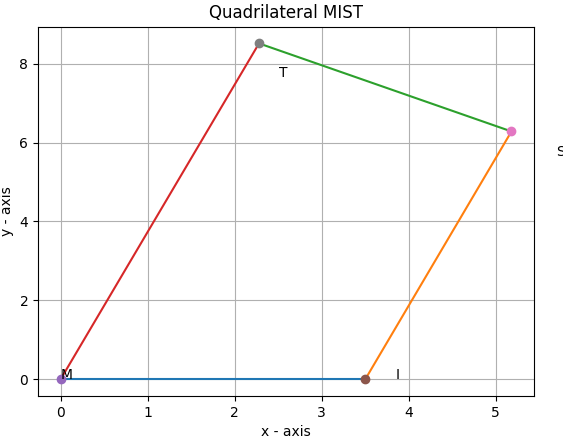
\includegraphics[ width=\columnwidth]{plot.png}
\caption{Quadrilateral MIST}
\label{plt}	
\end{figure}

\end{document}